\documentclass[tikz,border=5pt]{standalone}

\usetikzlibrary{automata, positioning, arrows.meta}

\begin{document}

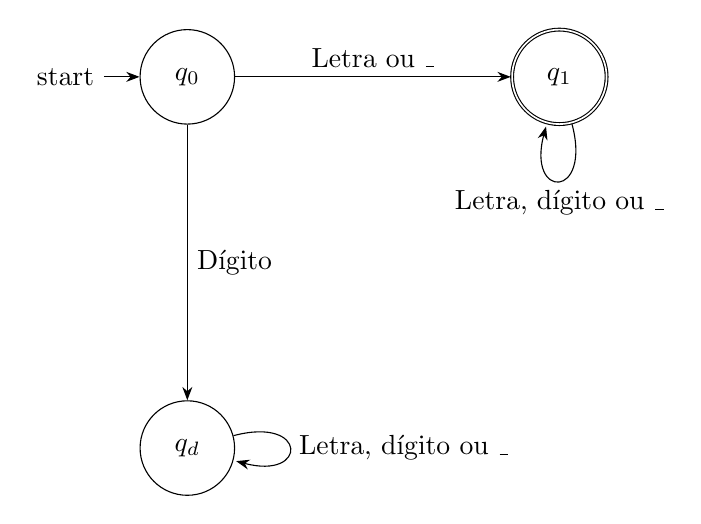
\begin{tikzpicture}[
    ->,
    >=Stealth,
    node distance=3.5cm,
    every state/.style={
        draw,
        circle,
        minimum size=1.2cm
    }
]

\node[state, initial] (q0) {$q_0$};
\node[state, accepting, right=of q0] (q1) {$q_1$};
\node[state, below=of q0] (qd) {$q_d$};

\path
(q0) edge[above] node{Letra ou \_} (q1)
(q0) edge[right] node{Dígito} (qd)
(q1) edge[loop below] node{Letra, dígito ou \_} ()
(qd) edge[loop right] node{Letra, dígito ou \_} ();

\end{tikzpicture}

\end{document}
